\clearpage

\section{Data vs. MC Comparison in Preselection Region}
\label{sec:yields}

In this section we compare the data and MC samples passing the selection described in Sec.~\ref{sec:eventSelection}
In the following, the MC is reweighted to match the data distribution of number of reconstructed primary vertices.
%{\bf FIXME: UPDATE TO 5.1/fb VTX-REWEIGHTING, CURRENTLY USING OUTDATED FUNCTION}. 
The trigger efficiencies of Sec.~\ref{sec:datasets} are applied. In all plots, the last bin contains the overflow.

We begin by counting the inclusive Z yields. Here we require the presence of two selected leptons without
any additional requirements on jets or \MET. In Fig.~\ref{fig:dilmass} the distribution of dilepton invariant
mass in the ee and $\mu\mu$ channels is displayed. In Table~\ref{table:zyields} the yields for selected dilepton
events in the Z mass window are indicated. Good data vs. MC agreement is observed, within the systematic uncertainties
of integrated luminosity (4.5\%), trigger efficiency (3\%), \zjets\ and \ttbar\ cross sections.

\begin{figure}[hbt]
  \begin{center}
	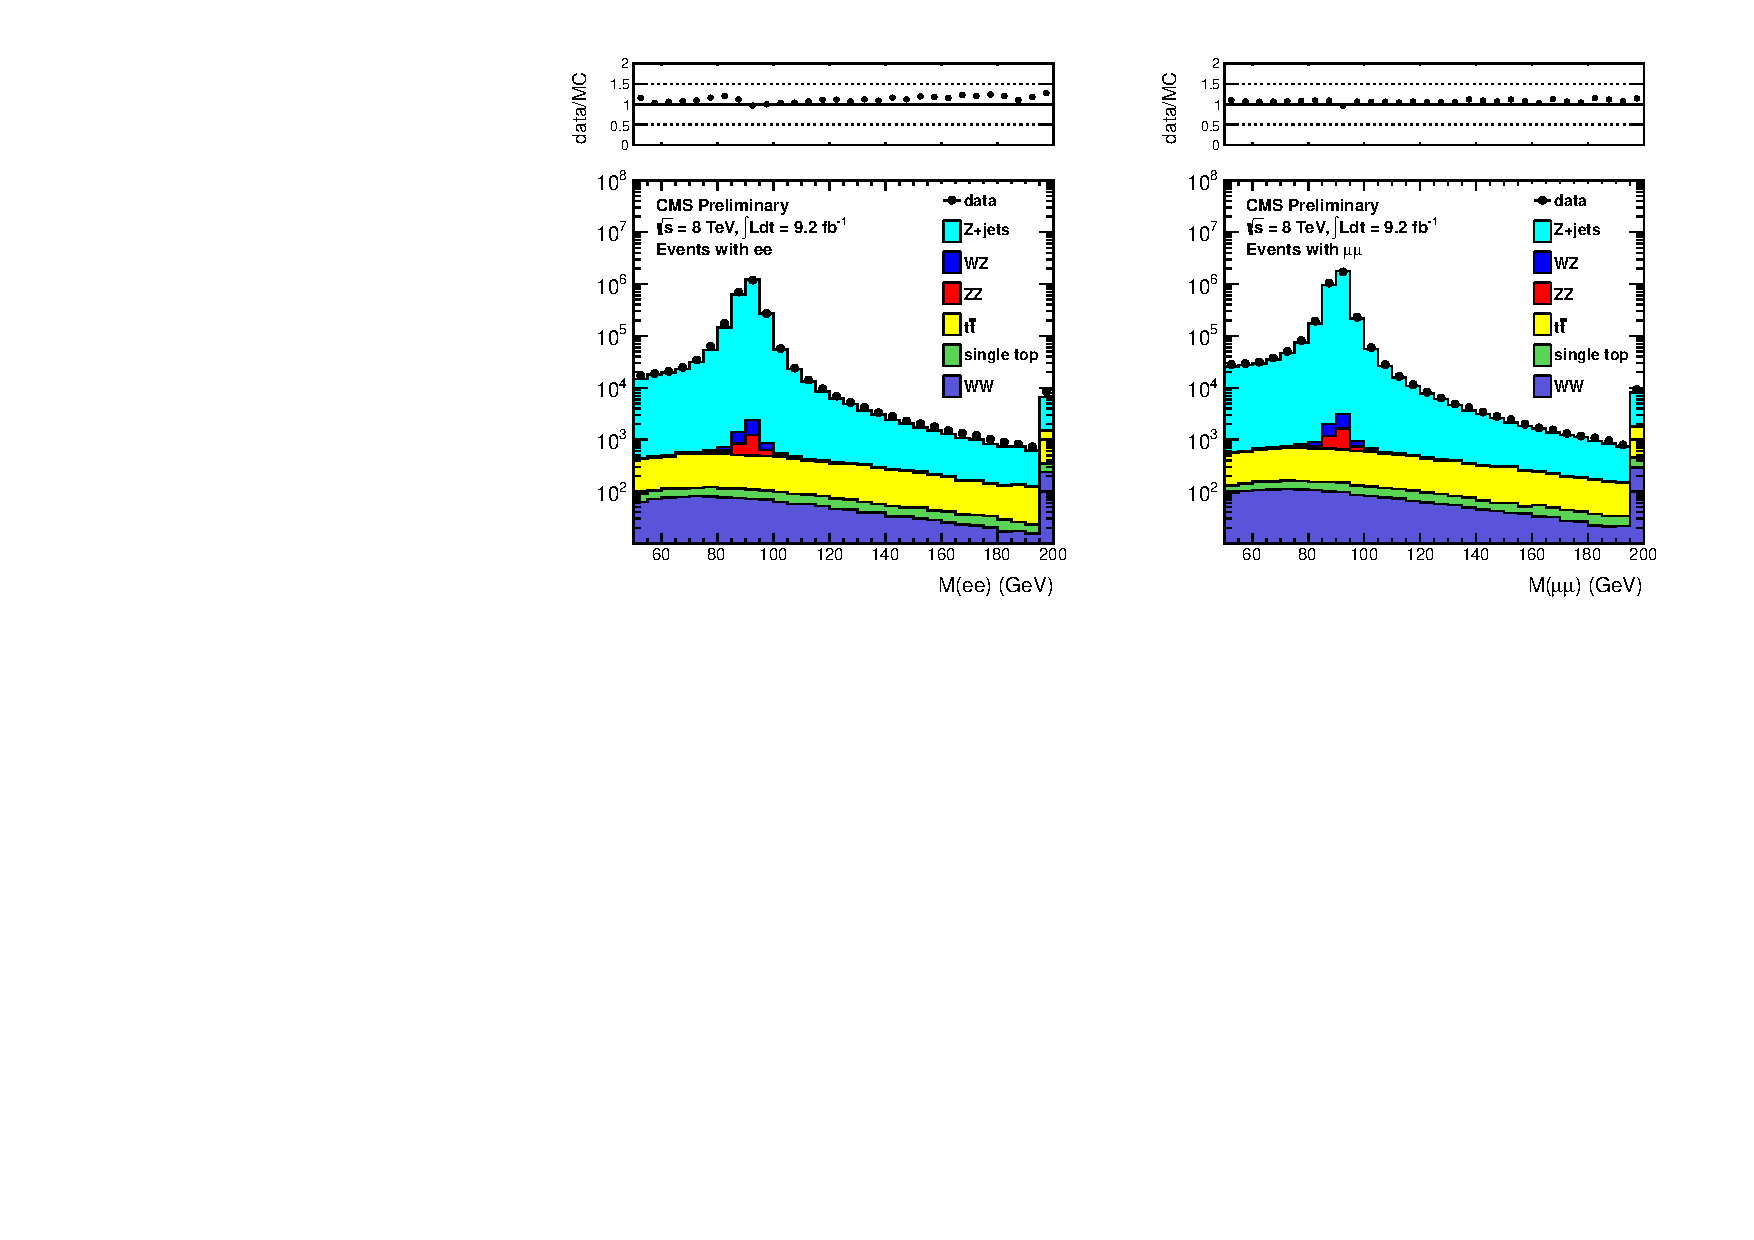
\includegraphics[width=1.0\linewidth]{plots/dilmass_92fb.pdf}
	\caption{
	  \label{fig:dilmass}\protect 
	  Dilepton mass distribution for events with two selected leptons
	  in the ee (left) and $\mu\mu$ (right) final states.}

%Loading babies at       : ../output/V00-01-04
%Using selection         : ((((isdata==0 || (run<197556 || run>198913))&&(((leptype==0 && (ee==1 || isdata==0))||(leptype==1 && (mm==1 || isdata==0)))||(leptype==2 && (em==1||me==1||isdata=%=0))))&&(csc==0 && hbhe==1 && hcallaser==1 && ecaltp==1 && trkfail==1 && eebadsc==1 && hbhenew==1))&&(lep1.pt()>20.0 && lep2.pt()>20.0))&&(dilmass>15.0)
%Using weight            : weight * 9.2 * trgeff * vtxweight
%Plotting var dilmass flavor ee
%compareDataMC : apply trigeff 1
%MC yield WW 1649.91
%MC yield single top 848.24
%MC yield ttbar 8915.92
%MC yield ZZ 1463.79
%MC yield WZ 2369.09
%SCALING ZJETS BY 111/946
%MC yield zjets 2546343.02
%MC total yield 2561590.00
%data yield 2.6608e+06
%Plotting var dilmass flavor mm
%compareDataMC : apply trigeff 1
%Warning in <TROOT::Append>: Replacing existing TH1: htemp (Potential memory leak).
%MC yield WW 2184.16
%MC yield single top 1099.46
%MC yield ttbar 11145.76
%MC yield ZZ 1922.01
%MC yield WZ 3077.27
%SCALING ZJETS BY 111/946
%MC yield zjets 3498798.71
%MC total yield 3518227.25
%data yield 3.60178e+06

  \end{center}
\end{figure}


\begin{table}[htb]
\begin{center}
\caption{\label{table:zyields} Data and Monte Carlo yields for events with two selected leptons in the Z mass window. }
\begin{tabular}{lccccc}
\hline
\hline
              Sample   &                ee   &            $\mu\mu$   &              e$\mu$   &         total         \\
\hline

%Loading babies at       : ../output/V00-01-04
%Using selection         : (((((isdata==0 || (run<197556 || run>198913))&&(((leptype==0 && (ee==1 || isdata==0))||(leptype==1 && (mm==1 || isdata==0)))||(leptype==2 && (em==1||me==1||isdata==0))))&&(csc==0 && hbhe==1 && hcallaser==1 && ecaltp==1 && trkfail==1 && eebadsc==1 && hbhenew==1))&&(lep1.pt()>20.0 && lep2.pt()>20.0))&&(dilmass>15.0))&&(dilmass>81 && dilmass<101)
%Using weight            : weight * 9.2 * trgeff * vtxweight

         \zjets   &22662501 $\pm$ 1660   &3125059 $\pm$ 1873   &1082 $\pm$ 35.8   &5392392 $\pm$ 2503  \\
           \ttbar   &1579.1 $\pm$ 22.6   &1998.3 $\pm$ 24.4   &3592.2 $\pm$ 33.5   &7169.5 $\pm$ 47.2  \\
             WW   &290.6 $\pm$ 2.9   &387.2 $\pm$ 3.3   &671.2 $\pm$ 4.4   &1349.0 $\pm$ 6.2  \\
             WZ   &2052.6 $\pm$ 3.6   &2686.9 $\pm$ 3.9   & 54.1 $\pm$ 0.5   &4793.5 $\pm$ 5.3  \\
             ZZ   &1294.6 $\pm$ 2.7   &1708.5 $\pm$ 3.0   &  5.2 $\pm$ 0.1   &3008.3 $\pm$ 4.0  \\
     single top   &150.0 $\pm$ 5.9   &192.6 $\pm$ 6.4   &332.9 $\pm$ 8.6   &675.5 $\pm$ 12.2  \\
\hline
      total SM MC   &2271617 $\pm$ 1661   &3132032 $\pm$ 18723   &5738 $\pm$ 50.0   &5409387 $\pm$ 2503  \\
\hline
           data   &        2329993   &        3169480   &           6182   &        5505655  \\
\hline
\hline
\end{tabular}
\end{center}
\end{table}

\clearpage

We next define the preselection region for the inclusive search using the following requirements:
\begin{itemize}
\item Number of jets $\geq$ 2;
\item Same flavor dileptons (opposite flavor yields will be shown since they are used in data for the FS background estimation);
\item Dilepton invariant mass $81<m_{\ell\ell}<101$ GeV.
\end{itemize}

The dilepton mass distributions in the preselection region of the inclusive search (without the dilepton mass requirement applied) 
for the ee and $\mu\mu$ final states are shown in Figure~\ref{fig:dilmass_2j}. In Table~\ref{table:zyields_2j} the data and MC yields 
in thepreselection region are indicated. Good data vs. MC agreement is observed.


\begin{figure}[hbt]
  \begin{center}
	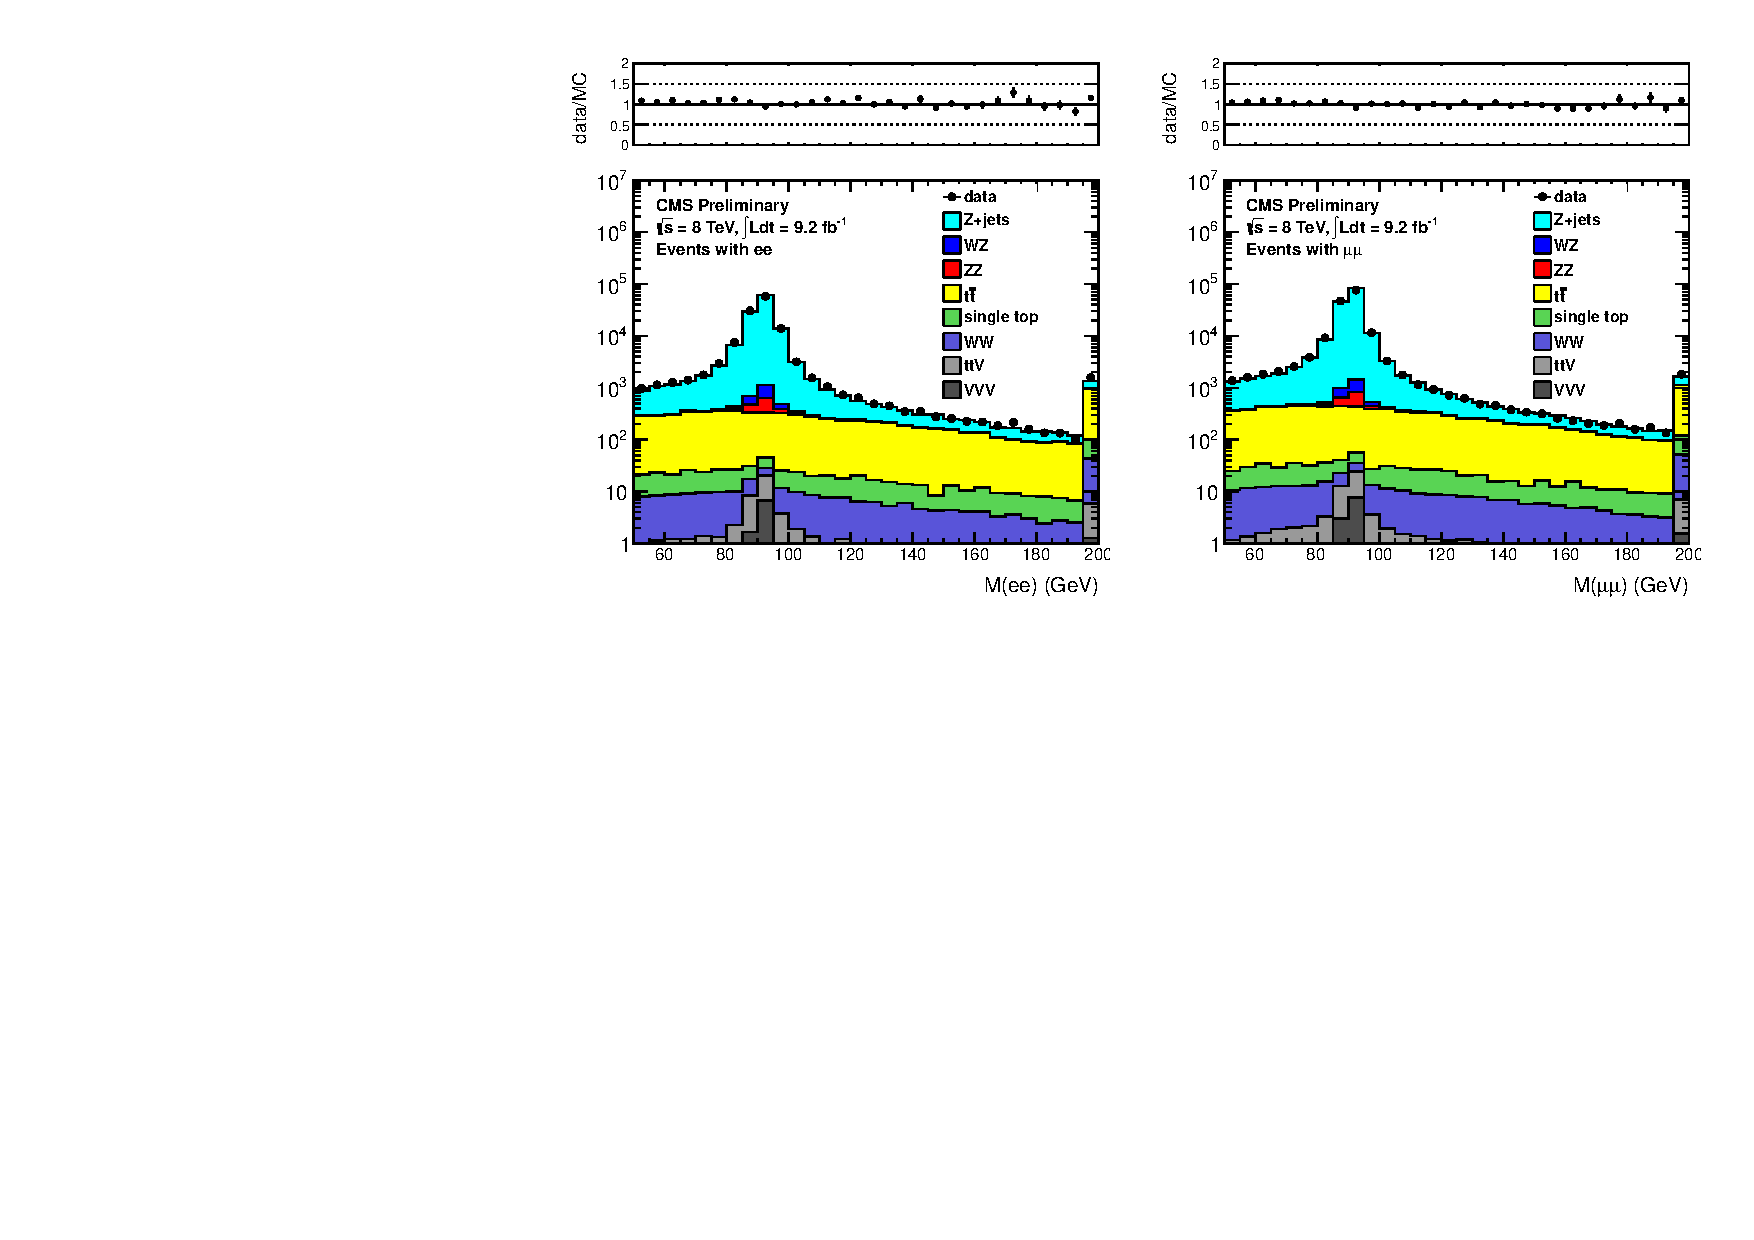
\includegraphics[width=1.0\linewidth]{plots/dilmass_2jets_92fb.pdf}
	\caption{
	  \label{fig:dilmass_2j}\protect 
	  Dilepton mass distribution for events in the preselection region of the inclusive search
	  in the ee (left) and $\mu\mu$ (right) final states.}

%Loading babies at       : ../output/V00-01-04
%-------------------------------------
%USING SKIMMED SAMPLES WITH NJETS >= 2
%-------------------------------------

%Using selection         : (((((isdata==0 || (run<197556 || run>198913))&&(((leptype==0 && (ee==1 || isdata==0))||(leptype==1 && (mm==1 || isdata==0)))||(leptype==2 && (em==1||me==1||isdata==0))))&&(csc==0 && hbhe==1 && hcallaser==1 && ecaltp==1 && trkfail==1 && eebadsc==1 && hbhenew==1))&&(lep1.pt()>20.0 && lep2.pt()>20.0))&&(dilmass>15.0))&&(njets>=2)
%Using weight            : weight * 9.2 * trgeff * vtxweight
%Plotting var dilmass flavor ee
%compareDataMC : apply trigeff 1
%MC yield VVV 13.81
%MC yield ttV 49.00
%MC yield WW 199.47
%MC yield single top 361.65
%MC yield ttbar 6867.43
%MC yield ZZ 600.93
%MC yield WZ 977.68
%SCALING ZJETS BY 111/946
%MC yield zjets 122957.78
%MC total yield 132027.75
%data yield 132109
%Plotting var dilmass flavor mm
%compareDataMC : apply trigeff 1
%Warning in <TROOT::Append>: Replacing existing TH1: htemp (Potential memory leak).
%MC yield VVV 17.13
%MC yield ttV 61.05
%MC yield WW 256.46
%MC yield single top 462.60
%MC yield ttbar 8583.48
%MC yield ZZ 778.67
%MC yield WZ 1252.40
%SCALING ZJETS BY 111/946
%MC yield zjets 164795.65
%MC total yield 176207.44
%data yield 171558

  \end{center}
\end{figure}

\begin{table}[htb]
\begin{center}
\caption{\label{table:zyields_2j} Data and MC yields in the preselection region of the inclusive search.
}
\begin{tabular}{lccccc}
\hline
\hline
         Sample   &           ee   &       $\mu\mu$   &         e$\mu$   &            total  \\
\hline


%Loading babies at       : ../output/V00-01-04
%-------------------------------------
%USING SKIMMED SAMPLES WITH NJETS >= 2
%-------------------------------------

%Using selection         : ((((((isdata==0 || (run<197556 || run>198913))&&(((leptype==0 && (ee==1 || isdata==0))||(leptype==1 && (mm==1 || isdata==0)))||(leptype==2 && (em==1||me==1||isdata==0))))&&(csc==0 && hbhe==1 && hcallaser==1 && ecaltp==1 && trkfail==1 && eebadsc==1 && hbhenew==1))&&(lep1.pt()>20.0 && lep2.pt()>20.0))&&(dilmass>15.0))&&(njets>=2))&&(dilmass>81 && dilmass<101)
%Using weight            : weight * 9.2 * trgeff * vtxweight

         \zjets   &108778.2 $\pm$ 358.0   &145999.4 $\pm$ 398.7   & 59.7 $\pm$ 8.3   &254837.4 $\pm$ 535.9  \\
         \ttbar   &1220.9 $\pm$ 19.9   &1544.7 $\pm$ 21.4   &2788.1 $\pm$ 29.5   &5553.8 $\pm$ 41.5  \\
             WW   & 32.7 $\pm$ 1.0   & 42.5 $\pm$ 1.1   & 74.7 $\pm$ 1.4   &149.9 $\pm$ 2.0  \\
             WZ   &853.0 $\pm$ 2.4   &1100.8 $\pm$ 2.6   & 10.7 $\pm$ 0.2   &1964.4 $\pm$ 3.5  \\
             ZZ   &532.5 $\pm$ 1.8   &692.6 $\pm$ 2.0   &  1.2 $\pm$ 0.0   &1226.3 $\pm$ 2.7  \\
     single top   & 60.4 $\pm$ 3.7   & 73.1 $\pm$ 3.9   &131.8 $\pm$ 5.4   &265.3 $\pm$ 7.6  \\
            ttV   & 25.9 $\pm$ 0.5   & 32.2 $\pm$ 0.5   &  9.4 $\pm$ 0.3   & 67.5 $\pm$ 0.8  \\
            VVV   &  9.2 $\pm$ 0.1   & 11.6 $\pm$ 0.2   &  1.6 $\pm$ 0.1   & 22.5 $\pm$ 0.2  \\
\hline
      tot SM MC   &111512.9 $\pm$ 358.6   &149497.0 $\pm$ 399.3   &3077.2 $\pm$ 31.1   &264087.1 $\pm$ 537.6  \\
\hline
           data   &         110325   &         144122   &           2966   &         257413  \\
\hline
\hline

\end{tabular}
\end{center}
\end{table}


\clearpage

We next define the preselection region for the targeted search by adding the following requirements:
\begin{itemize}
\item Veto events containing a b-tagged jet;
\item Dijet invariant mass $70<m_{jj}<110$ GeV;
\item Veto events containing a third selected lepton (electron or muon) with \pt $>$ 10 GeV; 
\end{itemize}

The rejection of events with a b-tagged jet strongly suppresses the \ttbar\ background, which is the dominant background in the inclusive search
after requiring large \MET. The requirement that the jet pair is consistent with originating from W/Z decay is motivated by the fact that we are 
searching for signatures producing V(jj)Z($\ell\ell$)+\MET; this requirement suppresses the \zjets\ and \ttbar\ backgrounds. The veto of events
containting a third electron or muon suppresses the WZ background, and also serves to make this analyis exclusive with respect to searches in
the trilepton final state.

The dilepton mass distributions in the preselection region of the targeted search (without the dilepton mass requirement applied) 
for the ee and $\mu\mu$ final states are shown in Figure~\ref{fig:dilmass_2j_targeted}. In Table~\ref{table:zyields_2j_targeted} 
the data and MC yields in the preselection region are indicated. Good data vs. MC agreement is observed.
We also show the distribution of dijet mass in the targeted preselection (with the requirement on this quantity removed) in Fig.~\ref{fig:mjj},
which demonstrates that the MC does a reasonable job of modeling this quantity.

%-------------------------------------
% veto b-jets with CSV MEDIUM 
%-------------------------------------

\begin{figure}[hbt]
  \begin{center}
	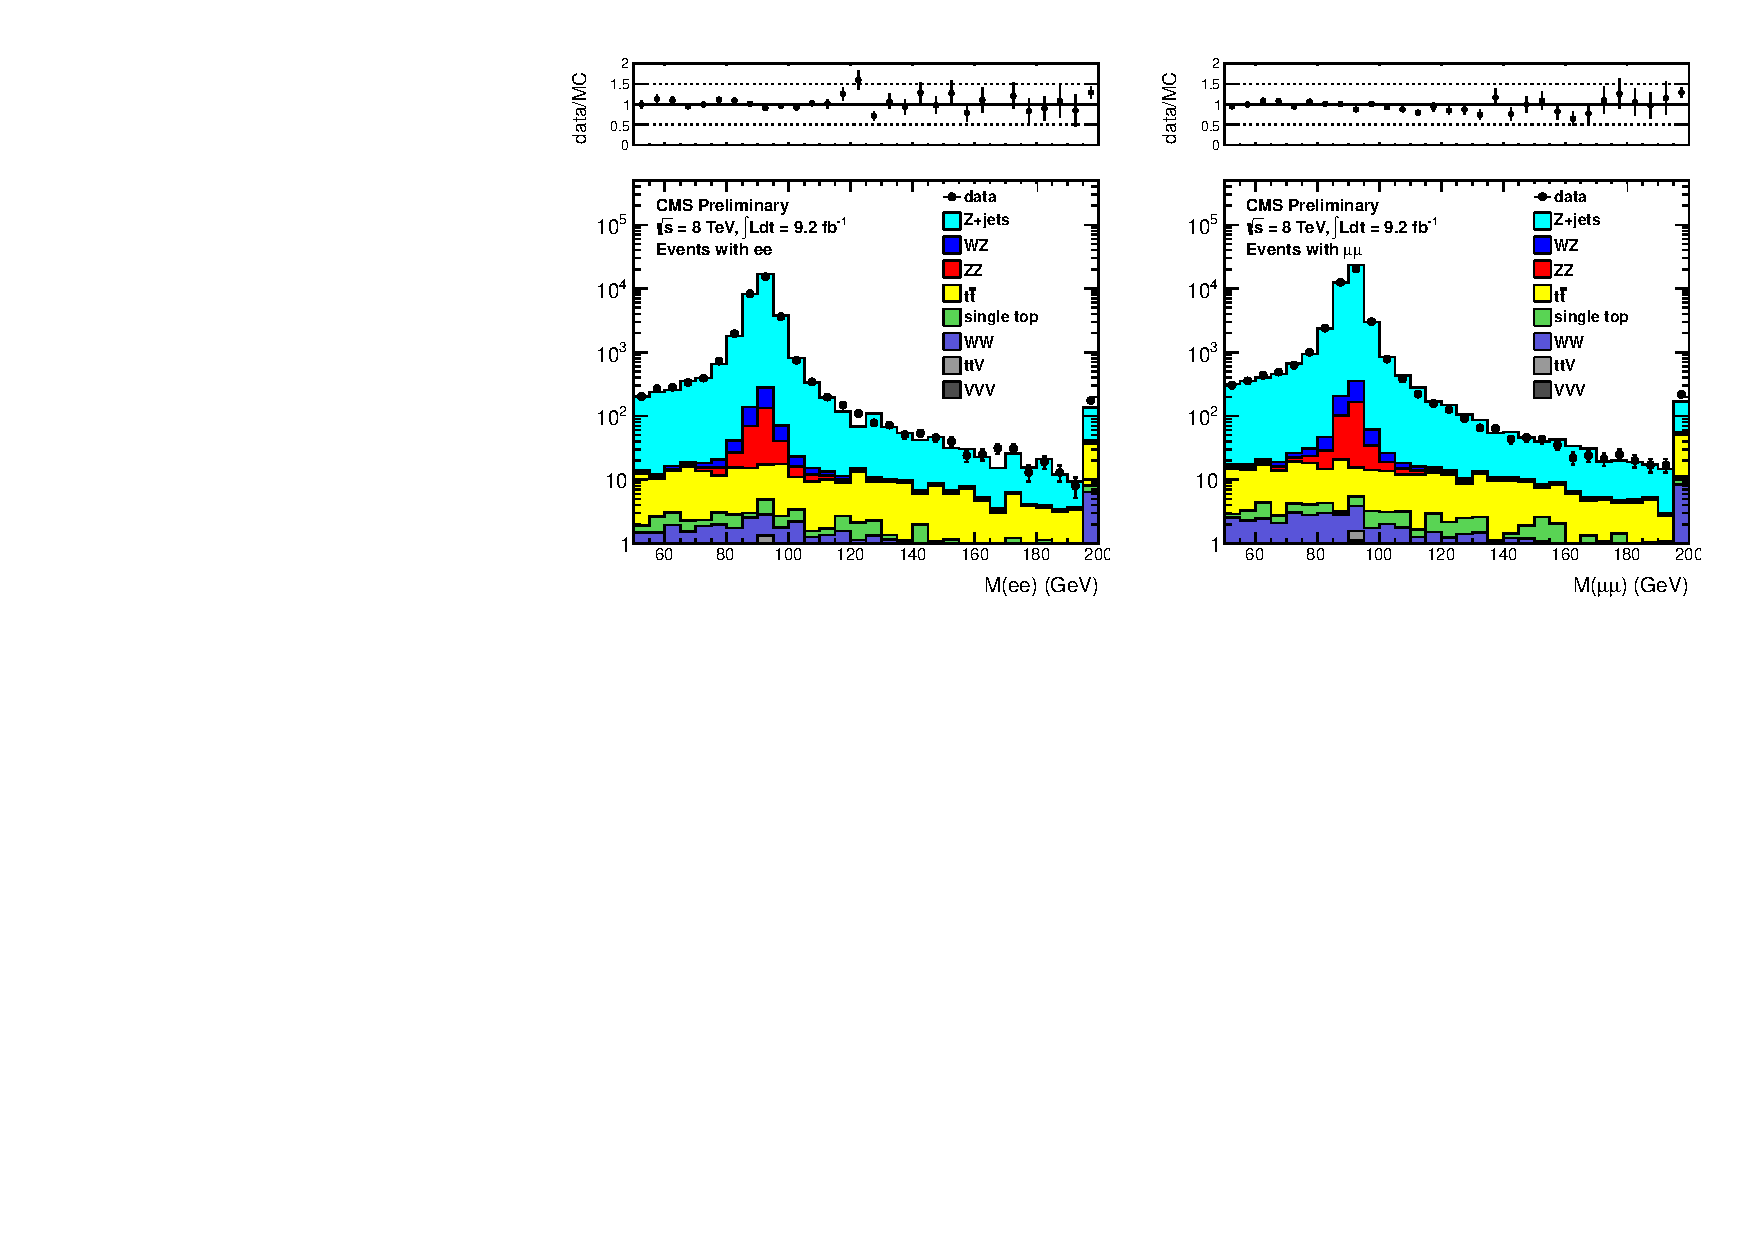
\includegraphics[width=1.0\linewidth]{plots/dilmass_2jets_92fb_bvetoMedium.pdf}
	\caption{
	  \label{fig:dilmass_2j_targeted}\protect 
	  Dilepton mass distribution for events in the preselection region of the targeted search
	  in the ee (left) and $\mu\mu$ (right) final states.}

%Loading babies at       : ../output/V00-01-04
%-------------------------------------
%USING SKIMMED SAMPLES WITH NJETS >= 2
%-------------------------------------

%Using selection         : ((((((((isdata==0 || (run<197556 || run>198913))&&(((leptype==0 && (ee==1 || isdata==0))||(leptype==1 && (mm==1 || isdata==0)))||(leptype==2 && (em==1||me==1||isdata==0))))&&(csc==0 && hbhe==1 && hcallaser==1 && ecaltp==1 && trkfail==1 && eebadsc==1 && hbhenew==1))&&(lep1.pt()>20.0 && lep2.pt()>20.0))&&(dilmass>15.0))&&(njets>=2))&&(nbcsvm==0))&&(mjj>70.0 && mjj<110.0))&&(nlep==2)
%Using weight            : weight * 9.2 * trgeff * vtxweight
%Plotting var dilmass flavor ee
%compareDataMC : apply trigeff 1
%MC yield VVV 2.50
%MC yield ttV 1.67
%MC yield WW 39.56
%MC yield single top 20.55
%MC yield ttbar 251.44
%MC yield ZZ 229.80
%MC yield WZ 297.15
%SCALING ZJETS BY 111/946
%MC yield zjets 33980.93
%MC total yield 34823.60
%data yield 33621
%Plotting var dilmass flavor mm
%compareDataMC : apply trigeff 1
%Warning in <TROOT::Append>: Replacing existing TH1: htemp (Potential memory leak).
%MC yield VVV 3.14
%MC yield ttV 1.71
%MC yield WW 51.07
%MC yield single top 28.09
%MC yield ttbar 289.65
%MC yield ZZ 296.84
%MC yield WZ 385.48
%SCALING ZJETS BY 111/946
%MC yield zjets 45992.12
%MC total yield 47048.08
%data yield 44092

  \end{center}
\end{figure}

\begin{table}[htb]
\begin{center}
\caption{\label{table:zyields_2j_targeted} Data and MC yields in the preselection region of the targeted search.
}
\begin{tabular}{lccccc}
\hline
\hline
         Sample   &           ee   &       $\mu\mu$   &         e$\mu$   &            total  \\
\hline

%Loading babies at       : ../output/V00-01-04
%-------------------------------------
%USING SKIMMED SAMPLES WITH NJETS >= 2
%-------------------------------------

%Using selection         : (((((((((isdata==0 || (run<197556 || run>198913))&&(((leptype==0 && (ee==1 || isdata==0))||(leptype==1 && (mm==1 || isdata==0)))||(leptype==2 && (em==1||me==1||is%data==0))))&&(csc==0 && hbhe==1 && hcallaser==1 && ecaltp==1 && trkfail==1 && eebadsc==1 && hbhenew==1))&&(lep1.pt()>20.0 && lep2.pt()>20.0))&&(dilmass>15.0))&&(njets>=2))&&(nbcsvm==0))&&(%mjj>70.0 && mjj<110.0))&&(nlep==2))&&(dilmass>81 && dilmass<101)
%Using weight            : weight * 9.2 * trgeff * vtxweight

         \zjets   &30033.0 $\pm$ 186.9   &40552.4 $\pm$ 208.9   & 12.9 $\pm$ 3.7   &70598.3 $\pm$ 280.4  \\
         \ttbar   & 50.5 $\pm$ 4.1   & 49.1 $\pm$ 3.8   &105.1 $\pm$ 5.7   &204.7 $\pm$ 8.0  \\
             WW   &  6.8 $\pm$ 0.4   &  8.6 $\pm$ 0.5   & 15.9 $\pm$ 0.7   & 31.3 $\pm$ 0.9  \\
             WZ   &260.7 $\pm$ 1.3   &339.8 $\pm$ 1.4   &  1.7 $\pm$ 0.1   &602.2 $\pm$ 2.0  \\
             ZZ   &204.2 $\pm$ 1.1   &264.0 $\pm$ 1.2   &  0.2 $\pm$ 0.0   &468.4 $\pm$ 1.7  \\
     single top   &  4.7 $\pm$ 1.1   &  5.0 $\pm$ 1.0   &  8.5 $\pm$ 1.3   & 18.2 $\pm$ 2.0  \\

            ttV   &  0.7 $\pm$ 0.1   &  0.8 $\pm$ 0.1   &  0.4 $\pm$ 0.1   &  2.0 $\pm$ 0.1  \\
            VVV   &  1.4 $\pm$ 0.1   &  1.8 $\pm$ 0.1   &  0.4 $\pm$ 0.0   &  3.6 $\pm$ 0.1  \\
\hline
      tot SM MC   &30562.0 $\pm$ 187.0   &41221.5 $\pm$ 208.9   &145.2 $\pm$ 7.0   &71928.6 $\pm$ 280.5  \\
\hline
           data   &          29183   &          38388   &            120   &          67691  \\
\hline
\hline

\end{tabular}
\end{center}
\end{table}



\begin{comment}

%-------------------------------------
% veto b-jets with CSV LOOSE 
%-------------------------------------

\begin{figure}[hbt]
  \begin{center}
	\includegraphics[width=1.0\linewidth]{plots/dilmass_2jets_92fb_bvetoLoose.pdf}
	\caption{
	  \label{fig:dilmass_2j_targeted}\protect 
	  Dilepton mass distribution for events in the preselection region of the targeted search
	  in the ee (left) and $\mu\mu$ (right) final states.}

%Loading babies at       : ../output/V00-01-04
%-------------------------------------
%USING SKIMMED SAMPLES WITH NJETS >= 2
%-------------------------------------

%Using selection         : ((((((((isdata==0 || (run<197556 || run>198913))&&(((leptype==0 && (ee==1 || isdata==0))||(leptype==1 && (mm==1 || isdata==0)))||(leptype==2 && (em==1||me==1||isdata==0))))&&(csc==0 && hbhe==1 && hcallaser==1 && ecaltp==1 && trkfail==1 && eebadsc==1 && hbhenew==1))&&(lep1.pt()>20.0 && lep2.pt()>20.0))&&(dilmass>15.0))&&(njets>=2))&&(nbcsvl==0))&&(mjj>70.0 && mjj<110.0))&&(nlep==2)
%Using weight            : weight * 9.2 * trgeff * vtxweight
%Plotting var dilmass flavor ee
%compareDataMC : apply trigeff 1
%MC yield VVV 1.69
%MC yield ttV 0.71
%MC yield WW 29.99
%MC yield single top 10.71
%MC yield ttbar 98.96
%MC yield ZZ 160.28
%MC yield WZ 201.63
%SCALING ZJETS BY 111/946
%MC yield zjets 26365.25
%MC total yield 26869.22
%data yield 24722
%Plotting var dilmass flavor mm
%compareDataMC : apply trigeff 1
%Warning in <TROOT::Append>: Replacing existing TH1: htemp (Potential memory leak).
%MC yield VVV 2.05
%MC yield ttV 0.70
%MC yield WW 38.74
%MC yield single top 13.48
%MC yield ttbar 104.95
%MC yield ZZ 206.22
%MC yield WZ 262.27
%SCALING ZJETS BY 111/946
%MC yield zjets 35489.85
%MC total yield 36118.25
%data yield 32393

  \end{center}
\end{figure}

\begin{table}[htb]
\begin{center}
\caption{\label{table:zyields_2j_targeted} Data and MC yields in the preselection region of the inclusive search.
}
\begin{tabular}{lccccc}
\hline
\hline
         Sample   &           ee   &       $\mu\mu$   &         e$\mu$   &            total  \\
\hline

%Loading babies at       : ../output/V00-01-04
%-------------------------------------
%USING SKIMMED SAMPLES WITH NJETS >= 2
%-------------------------------------

%Using selection         : (((((((((isdata==0 || (run<197556 || run>198913))&&(((leptype==0 && (ee==1 || isdata==0))||(leptype==1 && (mm==1 || isdata==0)))||(leptype==2 && (em==1||me==1||isdata==0))))&&(csc==0 && hbhe==1 && hcallaser==1 && ecaltp==1 && trkfail==1 && eebadsc==1 && hbhenew==1))&&(lep1.pt()>20.0 && lep2.pt()>20.0))&&(dilmass>15.0))&&(njets>=2))&&(nbcsvl==0))&&(mjj>70.0 && mjj<110.0))&&(nlep==2))&&(dilmass>81 && dilmass<101)
%Using weight            : weight * 9.2 * trgeff * vtxweight

\hline
         Sample   &           $ee$   &       $\mu\mu$   &         $e\mu$   &            tot  \\
\hline
SCALING ZJETS BY 111/946
          zjets   &23338.4 $\pm$ 164.1   &31251.5 $\pm$ 182.6   &  8.9 $\pm$ 3.1   &54598.8 $\pm$ 245.5  \\
             WZ   &176.4 $\pm$ 1.1   &231.1 $\pm$ 1.2   &  1.1 $\pm$ 0.1   &408.7 $\pm$ 1.6  \\
             ZZ   &142.3 $\pm$ 0.9   &183.2 $\pm$ 1.0   &  0.1 $\pm$ 0.0   &325.6 $\pm$ 1.4  \\
          ttbar   & 20.6 $\pm$ 2.5   & 15.5 $\pm$ 2.1   & 38.1 $\pm$ 3.4   & 74.2 $\pm$ 4.7  \\
     single top   &  2.3 $\pm$ 0.7   &  2.9 $\pm$ 0.7   &  4.5 $\pm$ 1.0   &  9.6 $\pm$ 1.4  \\
             WW   &  5.0 $\pm$ 0.4   &  6.8 $\pm$ 0.4   & 12.3 $\pm$ 0.6   & 24.2 $\pm$ 0.8  \\
            ttV   &  0.3 $\pm$ 0.1   &  0.3 $\pm$ 0.1   &  0.2 $\pm$ 0.0   &  0.8 $\pm$ 0.1  \\
            VVV   &  0.9 $\pm$ 0.0   &  1.1 $\pm$ 0.0   &  0.3 $\pm$ 0.0   &  2.3 $\pm$ 0.1  \\
\hline
      tot SM MC   &23686.1 $\pm$ 164.1   &31692.4 $\pm$ 182.6   & 65.7 $\pm$ 4.7   &55444.2 $\pm$ 245.5  \\
\hline
           data   &          21529   &          28265   &             53   &          49847  \\
\hline
\hline

\end{tabular}
\end{center}
\end{table}

\end{comment}


\clearpage

\begin{figure}[hbt]
  \begin{center}
	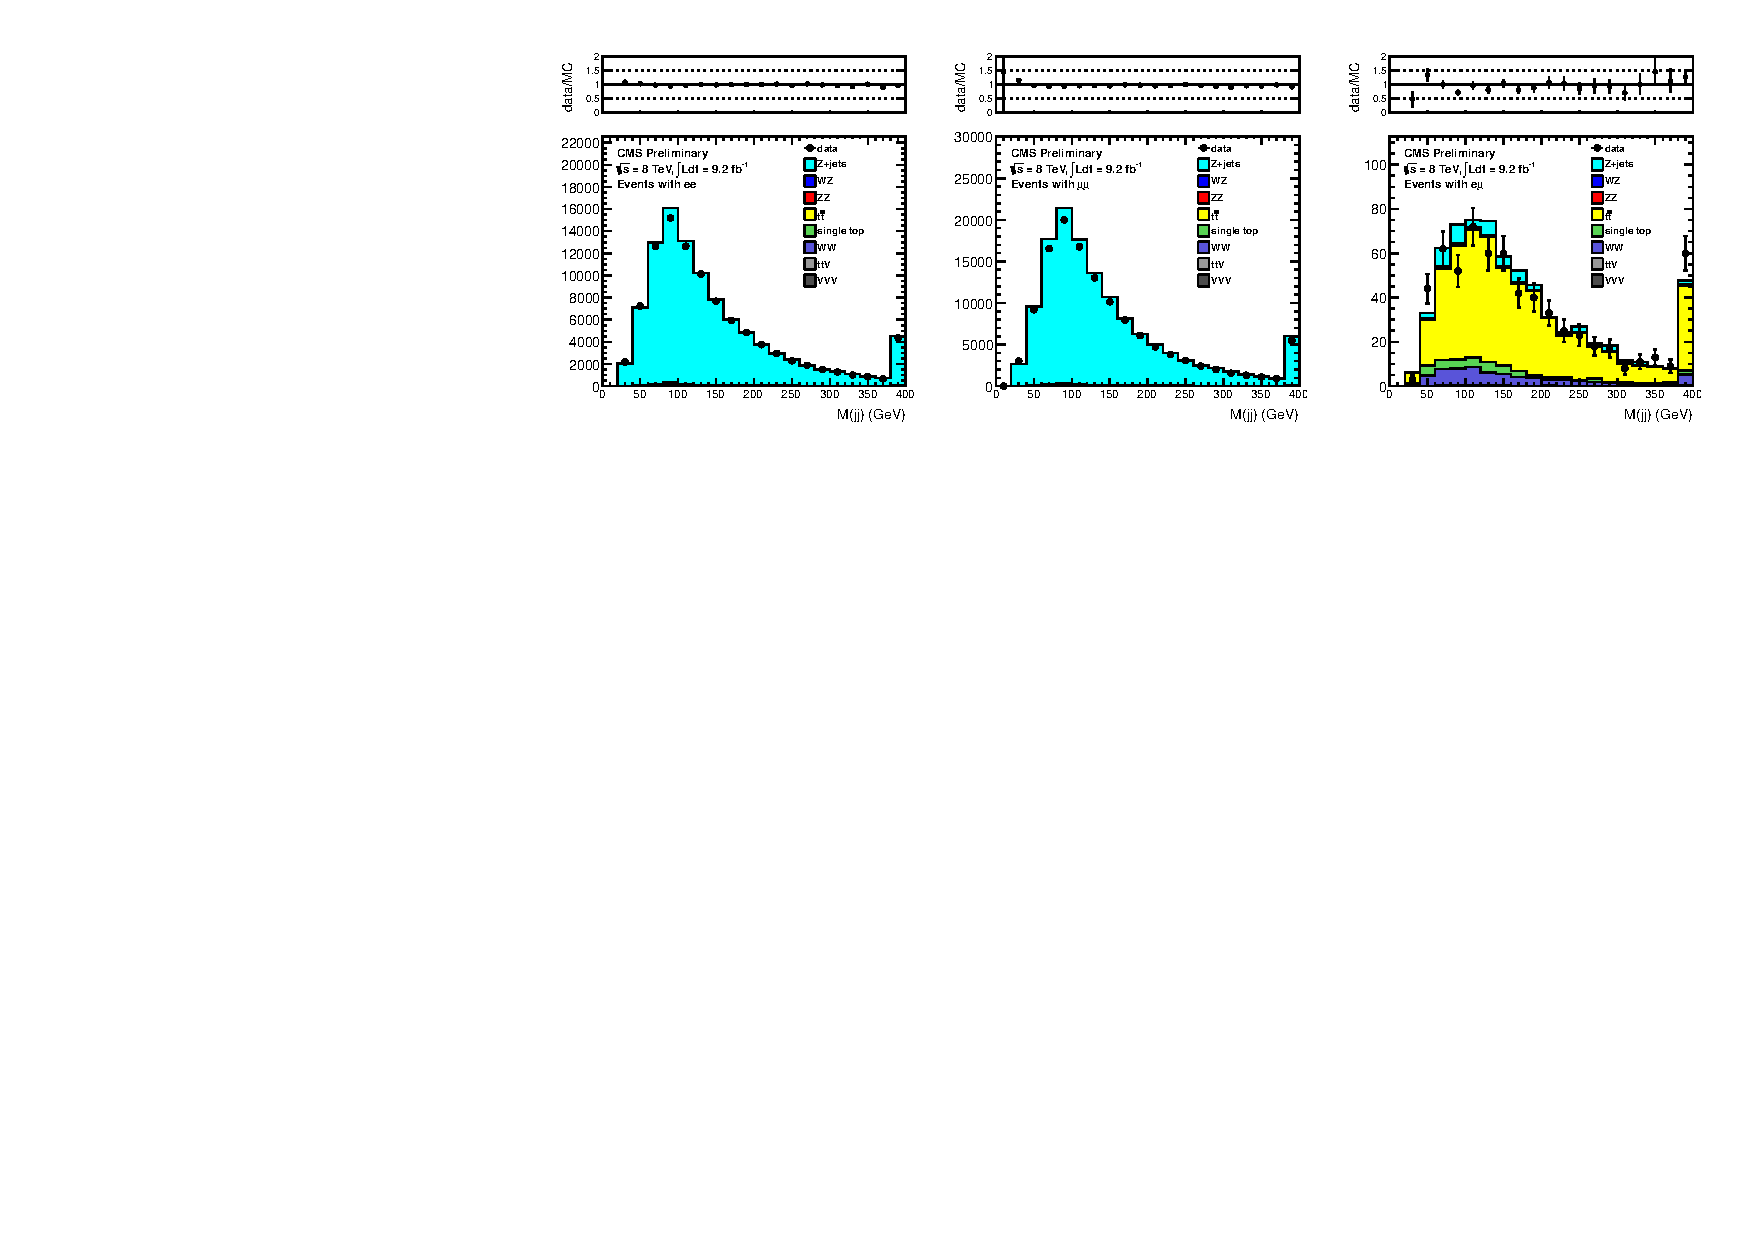
\includegraphics[width=1.0\linewidth]{plots/mjj_92fb.pdf}
	\caption{
	  \label{fig:mjj}\protect 
Distributions of dijet mass for the targeted preselection in the ee (left), $\mu\mu$ (middle) and e$\mu$ (right) final state.
}                   
  \end{center}
\end{figure}





